\section{Il problema del Disentanglement}
\label{sec:04_disentangling_dense_embeddings_with_sparse_autoencoders}

\epigraph{
    Essentially, all models are wrong, but some are useful.
}{George E. P. Box}

\newpage
\subsection{La Superposition Hypothesis}
\label{subsec:superposition_hypothesis}
Il Capitolo~\ref{sec:word_embeddings} si è concluso con un'osservazione problematica: gli embeddings prodotti da modelli come BERT catturano informazione semantica straordinariamente ricca, ma in forma \textit{opaca}. Le 768 dimensioni di un vettore BERT non corrispondono a proprietà linguistiche interpretabili—non esiste una dimensione per ``è un animale'', un'altra per ``esprime azione'', un'altra ancora per ``ha connotazione negativa''. L'informazione c'è, ma è distribuita in modo apparentemente indecifrabile.
Questa opacità non è un difetto accidentale dell'architettura, né una conseguenza di scelte progettuali subottimali. È invece il risultato di un fenomeno profondo che riguarda il modo stesso in cui le reti neurali rappresentano l'informazione: la \textbf{superposition}. Per comprendere questo fenomeno, è utile partire da una domanda: come \textit{vorremmo} che fossero organizzate le rappresentazioni neurali?
\subsubsection{Il mondo ideale: rappresentazioni disentangled}
Nel Capitolo~\ref{sec:interpretabilita_disentanglement} abbiamo introdotto il concetto di \textit{disentanglement}: una proprietà delle rappresentazioni latenti in cui ogni dimensione cattura esattamente un fattore di variazione dei dati. Applichiamo ora questa idea al contesto specifico dei modelli linguistici.
Immaginiamo una rete neurale ``ideale'' dal punto di vista dell'interpretabilità. In questa rete, ogni neurone—ogni singola dimensione dello spazio delle attivazioni—corrisponderebbe a esattamente un concetto semantico:
\begin{itemize}
    \item Il neurone 1 si attiva se e solo se l'input menziona un \textit{animale}
    \item Il neurone 2 si attiva se e solo se la frase esprime \textit{sentimento negativo}
    \item Il neurone 3 si attiva se e solo se il testo riguarda \textit{meccanica quantistica}
    \item Il neurone 4 si attiva se e solo se si parla di \textit{torta al cioccolato}
    \item E così via...
\end{itemize}
Questa configurazione è ciò che Wang et al.~\parencite{wang2024disentangledrepresentationlearning} definiscono una \textbf{rappresentazione disentangled}:
\begin{notebox}
\textbf{Rappresentazione Disentangled (ideale)}\\
Una rappresentazione si dice \textit{disentangled} quando esiste una corrispondenza biunivoca tra le dimensioni dello spazio latente e i fattori semantici sottostanti ai dati:
\begin{enumerate}
    \item Ogni dimensione (neurone) codifica \textbf{esattamente un} concetto
    \item Ogni concetto è catturato da \textbf{esattamente una} dimensione
\end{enumerate}
In termini formali, se $n$ è il numero di neuroni e $k$ il numero di concetti, una rappresentazione perfettamente disentangled richiede $n = k$.
\end{notebox}
In un mondo così organizzato, interpretare il modello sarebbe banale. Per sapere cosa la rete ha ``riconosciuto'' in un dato input, basterebbe osservare quali neuroni si sono attivati. Nessuna analisi sofisticata, nessuna tecnica di interpretabilità: la struttura stessa della rappresentazione renderebbe trasparente il funzionamento interno.
Modificare il comportamento del modello sarebbe altrettanto semplice. Se volessimo che la rete ignorasse il sentimento di una frase, basterebbe silenziare il neurone corrispondente. Se volessimo amplificare l'attenzione verso concetti culinari, basterebbe potenziare i neuroni dedicati a quel dominio.
Ma i modelli reali non funzionano così. E la ragione non è una limitazione ingegneristica—è qualcosa di più profondo.
\subsubsection{Il paradosso della capacità}
Consideriamo ora i numeri concreti. BERT-base, uno dei modelli linguistici più studiati, rappresenta ogni token con un vettore di 768 dimensioni. Questo significa 768 neuroni per ogni posizione nella sequenza—768 numeri che devono catturare tutto ciò che il modello ``sa'' su quella parola in quel contesto.
Ma cosa ``sa'' BERT? L'elenco è impressionante. Il modello dimostra di riconoscere entità come persone, luoghi, organizzazioni, opere e prodotti—migliaia di categorie—insieme a relazioni sintattiche quali soggetto-verbo, modificatore-testa e dipendenze a lunga distanza. Comprende proprietà semantiche come animatezza, concretezza, polarità emotiva e formalità, oltre a possedere conoscenza enciclopedica di fatti storici, relazioni geografiche e proprietà degli oggetti. Il modello cattura sfumature pragmatiche come ironia, understatement e registro linguistico, ed è competente in domini specialistici che spaziano dalla terminologia medica a quella legale, tecnica e scientifica.
Una stima conservativa suggerisce che un modello come BERT debba rappresentare \textit{decine di migliaia} di concetti distinti per esibire le capacità che osserviamo empiricamente. Probabilmente molti di più.
Ora il problema diventa evidente:
\begin{equation}
    768 \text{ neuroni} \quad \ll \quad \text{decine di migliaia di concetti}
\end{equation}
Se ogni concetto richiedesse un neurone dedicato—come nel mondo disentangled ideale—768 dimensioni permetterebbero al massimo 768 concetti. Ma BERT ne gestisce ordini di grandezza in più. I conti non tornano.
Eppure il modello funziona. Non solo funziona, ma raggiunge prestazioni straordinarie su una vasta gamma di compiti linguistici. Come è possibile?
La risposta a questo paradosso richiede di abbandonare un'assunzione implicita che abbiamo fatto finora—un'assunzione così naturale da sembrare ovvia, ma che si rivela essere il cuore del problema.\subsubsection{Neuroni e feature: una distinzione cruciale}
L'assunzione nascosta è questa: abbiamo implicitamente identificato i \textit{neuroni} con le \textit{feature}. Abbiamo ragionato come se ogni concetto dovesse ``abitare'' in un neurone dedicato, e ogni neurone potesse ospitare un solo concetto. Ma queste due entità—neuroni e feature—sono oggetti profondamente diversi.
\begin{notebox}
\textbf{Neuroni vs Feature}
\begin{itemize}
    \item Un \textbf{neurone} (o \textit{dimensione}) è un'unità computazionale della rete: un singolo valore numerico nello spazio delle attivazioni. I neuroni sono gli \textbf{assi} del sistema di coordinate—le direzioni ``cardinali'' lungo cui misuriamo le attivazioni. In BERT-base, ci sono 768 neuroni che definiscono gli assi $d_1, d_2, \dots, d_{768}$.    
    \item Una \textbf{feature} $f_i$ è un concetto semantico che vorremmo catturare: ``torta al cioccolato'', ``meccanica quantistica'', ``sentimento negativo''. Le feature sono le proprietà \textit{dei dati} che risultano utili per i compiti del modello—i ``fattori generativi'' della semantica.
\end{itemize}
\end{notebox}
La chiave per comprendere la superposition sta nel realizzare che \textit{le feature non devono necessariamente coincidere con gli assi}. Una feature può essere rappresentata come una \textbf{direzione arbitraria} nello spazio—un vettore che punta in una direzione qualsiasi, combinando più neuroni con pesi diversi. Indichiamo con $\mathbf{w}_i \in \mathbb{R}^{768}$ la direzione associata alla feature $f_i$ nello spazio di BERT.
Consideriamo un'analogia geografica, illustrata in Figura~\ref{fig:geographic_analogy}. Se dobbiamo descrivere la posizione di una città, possiamo usare le coordinate cardinali: ``100 km a Nord, 50 km a Est''. Gli assi Nord-Sud ed Est-Ovest sono i nostri ``neuroni''—le direzioni di riferimento del sistema. Ma nulla ci impedisce di descrivere la stessa posizione come ``112 km in direzione Nord-Nord-Est''. La direzione Nord-Nord-Est non coincide con nessun asse, ma è perfettamente definita come combinazione degli assi.
\begin{figure}[htbp]
    \centering
    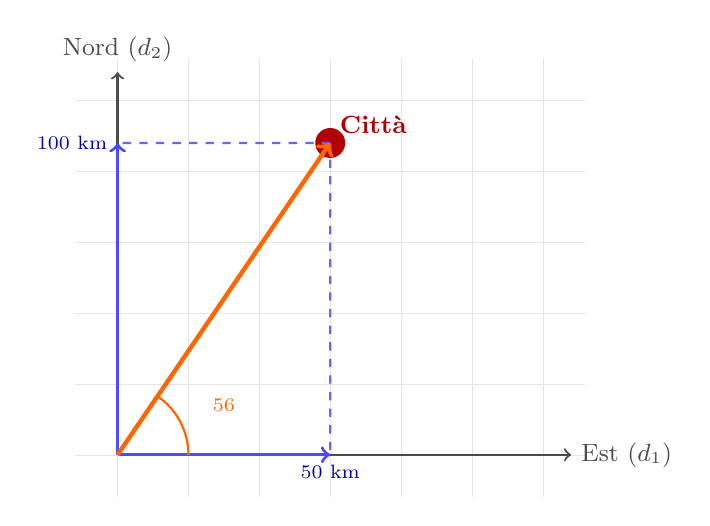
\begin{tikzpicture}[scale=1.8]
        % Griglia di sfondo
        \draw[gray!20, very thin, step=0.5] (-0.3,-0.3) grid (3.3,2.8);
                % Assi (neuroni)
        \draw[->, thick, black!70] (0,0) -- (3.2,0) node[right, font=\small] {Est ($d_1$)};
        \draw[->, thick, black!70] (0,0) -- (0,2.7) node[above, font=\small] {Nord ($d_2$)};
        
        % Punto di destinazione
        \coordinate (city) at (1.5, 2.2);
        \fill[red!70!black] (city) circle (3pt);
        \node[anchor=south west, font=\small\bfseries, red!70!black] at (city) {Città};
        
        % Componenti sugli assi (proiezioni tratteggiate)
        \draw[dashed, blue!60, thick] (city) -- (1.5, 0) node[below, font=\scriptsize, blue!70!black] {50 km};
        \draw[dashed, blue!60, thick] (city) -- (0, 2.2) node[left, font=\scriptsize, blue!70!black] {100 km};
        
        % Vettori componenti sugli assi
        \draw[->, very thick, blue!70] (0,0) -- (1.5, 0);
        \draw[->, very thick, blue!70] (0,0) -- (0, 2.2);
        
        % Direzione obliqua (la feature)
        \draw[->, ultra thick, orange!80!red] (0,0) -- (city);

        
        % Angolo
        \draw[orange!80!red, thick] (0.5,0) arc (0:56:0.5);
        \node[orange!80!red, font=\scriptsize] at (0.75, 0.35) {$56°$};
    \end{tikzpicture}
    \caption{Analogia geografica tra neuroni e feature. Gli assi cardinali (Nord, Est) rappresentano i neuroni: le direzioni di riferimento del sistema. La direzione Nord-Nord-Est rappresenta una feature: non coincide con nessun asse, ma è definita come loro combinazione ($100 \text{ km Nord} + 50 \text{ km Est} = 112 \text{ km NNE}$). In uno spazio bidimensionale esistono solo 2 assi, ma infinite direzioni.}
    \label{fig:geographic_analogy}
\end{figure}

\begin{notebox}
\textbf{Feature}\\
Una feature è una \textit{direzione} nello spazio vettoriale dei neuroni.
\end{notebox}
Allo stesso modo, una feature come $f_{\text{torta}}$ (``torta al cioccolato'') non deve necessariamente corrispondere all'asse $d_{42}$. Può essere rappresentata come una direzione obliqua $\mathbf{w}_{\text{torta}}$ nello spazio delle attivazioni:
\begin{equation}
    \mathbf{w}_{\text{torta}} = 0.7 \cdot \mathbf{d}_1 + 0.5 \cdot \mathbf{d}_2 - 0.3 \cdot \mathbf{d}_3 + \dots
\end{equation}
una combinazione di molti neuroni, nessuno dei quali ``significa'' torta al cioccolato in isolamento.
Questa osservazione apre una possibilità che il ragionamento precedente escludeva: \textit{se le feature sono direzioni e non assi, possiamo avere più feature che neuroni}. In uno spazio tridimensionale esistono solo tre assi, ma infinite direzioni. La domanda diventa: quante direzioni ``utili'' possiamo stipare in uno spazio a $n$ dimensioni?
\subsubsection{La geometria della superposition}
Torniamo al nostro esempio con neuroni e feature, ma questa volta ragioniamo geometricamente. Consideriamo uno spazio semplificato con soli due neuroni—due assi, $d_1$ e $d_2$—e vediamo cosa succede al variare del numero di feature da rappresentare.
\paragraph{Caso ideale: due feature, due neuroni.}
Supponiamo di avere esattamente due feature da rappresentare: $f_{\text{torta}}$ (``torta al cioccolato'') e $f_{\text{quant}}$ (``meccanica quantistica''). Con due neuroni a disposizione, possiamo assegnare a ciascuna feature un asse dedicato. Le direzioni $\mathbf{w}_{\text{torta}}$ e $\mathbf{w}_{\text{quant}}$ coincidono con gli assi:
\begin{equation}
    \mathbf{w}_{\text{torta}} = \begin{pmatrix} 1 \\ 0 \end{pmatrix} = \mathbf{d}_1, \qquad
    \mathbf{w}_{\text{quant}} = \begin{pmatrix} 0 \\ 1 \end{pmatrix} = \mathbf{d}_2
\end{equation}
Questa è una rappresentazione perfettamente \textit{disentangled}: ogni feature coincide con un asse. Le due direzioni sono \textbf{ortogonali}, il loro prodotto scalare è quindi pari a zero ($\mathbf{w}_{\text{torta}} \cdot \mathbf{w}_{\text{quant}} = 0$) e questo significa che sono completamente indipendenti.
In questa configurazione, l'embedding $\mathbf{x}$ di un input si scrive come semplice combinazione:
\begin{equation}
    \mathbf{x} = a_{\text{torta}} \cdot \mathbf{w}_{\text{torta}} + a_{\text{quant}} \cdot \mathbf{w}_{\text{quant}} = \begin{pmatrix} a_{\text{torta}} \\ a_{\text{quant}} \end{pmatrix}
\end{equation}
dove $a_{\text{torta}}$ e $a_{\text{quant}}$ sono le \textit{intensità} con cui ogni feature è presente nell'input (zero se la feature è assente, positiva se presente).
Interpretare $\mathbf{x}$ è banale: la prima coordinata ci dice direttamente quanto è attiva la feature $f_{\text{torta}}$, la seconda quanto è attiva $f_{\text{quant}}$. Nessuna ambiguità, nessuna interferenza. Questo è il mondo ideale in cui vorremmo vivere.
\begin{figure}[htbp]
    \centering
    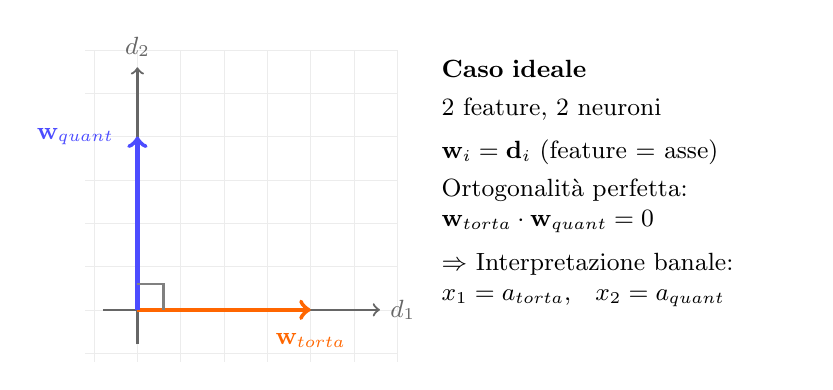
\begin{tikzpicture}[scale=2.2]
        % Griglia
        \draw[gray!15, very thin, step=0.25] (-0.3,-0.3) grid (1.5,1.5);        
        % Assi (neuroni)
        \draw[->, thick, black!60] (-0.2,0) -- (1.4,0) node[right, font=\small] {$d_1$};
        \draw[->, thick, black!60] (0,-0.2) -- (0,1.4) node[above, font=\small] {$d_2$};       
        % Feature allineate agli assi
        \draw[->, ultra thick, orange!80!red] (0,0) -- (1,0);
        \node[anchor=north, font=\small\bfseries, orange!80!red] at (1, -0.08) {$\mathbf{w}_{\text{torta}}$};        
        \draw[->, ultra thick, blue!70] (0,0) -- (0,1);
        \node[anchor=east, font=\small\bfseries, blue!70] at (-0.08, 1) {$\mathbf{w}_{\text{quant}}$};
        
        % Angolo retto
        \draw[thick, black!50] (0.15,0) -- (0.15,0.15) -- (0,0.15);
        
        % Etichetta
        \node[anchor=north west, font=\small, align=left, text width=4.5cm] at (1.7, 1.5) {
            \textbf{Caso ideale}\\[0.3em]
            2 feature, 2 neuroni\\[0.5em]
            $\mathbf{w}_i = \mathbf{d}_i$ (feature $=$ asse)\\[0.3em]
            Ortogonalità perfetta:\\
            $\mathbf{w}_{\text{torta}} \cdot \mathbf{w}_{\text{quant}} = 0$\\[0.5em]
            $\Rightarrow$ Interpretazione banale:\\
            $x_1 = a_{\text{torta}}$, \; $x_2 = a_{\text{quant}}$
        };
    \end{tikzpicture}
    \caption{Rappresentazione disentangled ideale. Con due feature e due neuroni, ogni direzione $\mathbf{w}_i$ coincide con un asse $\mathbf{d}_i$. Le coordinate di $\mathbf{x}$ indicano direttamente le intensità $a_i$ di ciascuna feature.}
    \label{fig:ideal_two_features}
\end{figure}

\paragraph{Il problema: tre feature, due neuroni.}
Aggiungiamo ora una terza feature: $f_{\text{ricetta}}$ (``ricetta di cucina''). Improvvisamente ci troviamo in difficoltà: lo spazio ha solo due assi, ma tre feature da rappresentare. Nella logica del mondo ideale, dovremmo rinunciare a una delle tre—non c'è spazio per tutte sugli assi.
Ma esiste un'alternativa. Se accettiamo che le direzioni $\mathbf{w}_i$ non debbano coincidere con gli assi, possiamo rappresentare tutte e tre le feature come \textit{direzioni} nel piano. La configurazione geometricamente ottimale è quella che le rende il più possibile ``separate''—il più possibile ortogonali, nei limiti del vincolo dimensionale.
In due dimensioni, la migliore disposizione per tre vettori unitari è quella che li distribuisce uniformemente: tre direzioni a 120° l'una dall'altra, come i vertici di un triangolo equilatero centrato nell'origine.

\begin{figure}[htbp]
    \centering
    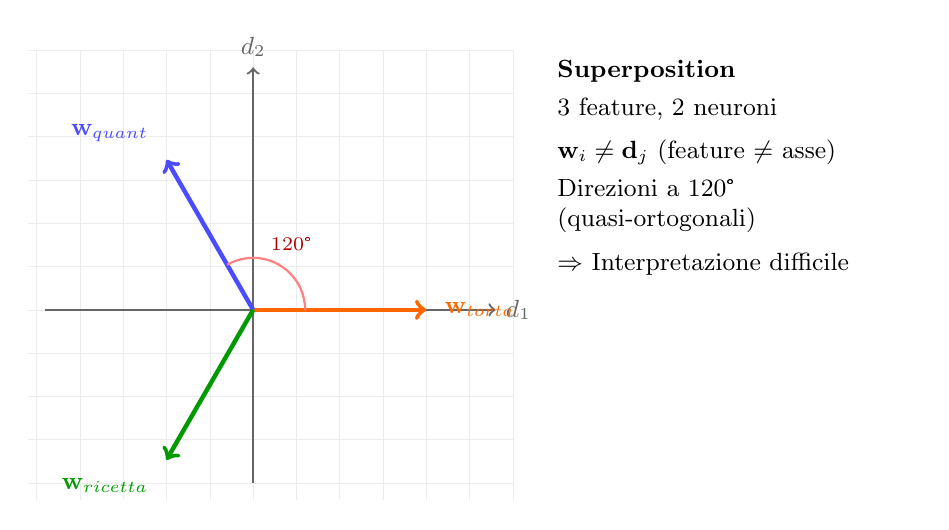
\begin{tikzpicture}[scale=2.2]
        % Griglia
        \draw[gray!15, very thin, step=0.25] (-1.3,-1.1) grid (1.5,1.5);
        
        % Assi (neuroni)
        \draw[->, thick, black!60] (-1.2,0) -- (1.4,0) node[right, font=\small] {$d_1$};
        \draw[->, thick, black!60] (0,-1.0) -- (0,1.4) node[above, font=\small] {$d_2$};
        
        % Tre feature a 120° (direzioni quasi-ortogonali)
        % w_torta: 0°
        \draw[->, ultra thick, orange!80!red] (0,0) -- (1,0);
        \node[anchor=west, font=\small\bfseries, orange!80!red] at (1.05, 0) {$\mathbf{w}_{\text{torta}}$};
        
        % w_quant: 120°
        \draw[->, ultra thick, blue!70] (0,0) -- ({cos(120)},{sin(120)});
        \node[anchor=south east, font=\small\bfseries, blue!70] at ({cos(120)-0.05},{sin(120)+0.05}) {$\mathbf{w}_{\text{quant}}$};
        
        % w_ricetta: 240°
        \draw[->, ultra thick, green!60!black] (0,0) -- ({cos(240)},{sin(240)});
        \node[anchor=north east, font=\small\bfseries, green!60!black] at ({cos(240)-0.05},{sin(240)-0.05}) {$\mathbf{w}_{\text{ricetta}}$};
        
        % Angoli
        \draw[red!50, thick] (0.3,0) arc (0:120:0.3);
        \node[red!70!black, font=\scriptsize] at (0.22, 0.38) {120°};
        
        % Etichetta
        \node[anchor=north west, font=\small, align=left, text width=4.5cm] at (1.7, 1.5) {
            \textbf{Superposition}\\[0.3em]
            3 feature, 2 neuroni\\[0.5em]
            $\mathbf{w}_i \neq \mathbf{d}_j$ (feature $\neq$ asse)\\[0.3em]
            Direzioni a 120°\\
            (quasi-ortogonali)\\[0.5em]
            $\Rightarrow$ Interpretazione difficile
        };
    \end{tikzpicture}
    \caption{Superposition: tre feature in due dimensioni. Le direzioni $\mathbf{w}_i$ non coincidono più con gli assi; sono disposte a 120° l'una dall'altra—la configurazione che massimizza la ``separazione'' nel piano.}
    \label{fig:superposition_three_features}
\end{figure}
Questa configurazione è ciò che Elhage et al.~\parencite{elhage2022superposition} chiamano \textbf{superposition}: la rete rappresenta più feature di quanti siano i neuroni disponibili, codificando le direzioni $\mathbf{w}_i$ come vettori quasi-ortogonali nello spazio delle attivazioni.
\begin{notebox}
\textbf{Superposition Hypothesis}\\
Le reti neurali rappresentano $m$ feature in uno spazio di $n$ dimensioni, con $m > n$, codificando ogni feature $f_i$ come una \textbf{direzione} (vettore unitario) $\mathbf{w}_i$ nello spazio delle attivazioni. Le direzioni sono scelte per essere il più possibile \textit{quasi-ortogonali}—indipendenti nei limiti del vincolo dimensionale. Il risultato è una rappresentazione compressa ma \textit{polisemantica}: ogni neurone partecipa alla codifica di molteplici feature.
\end{notebox}
\paragraph{L'opacità: direzioni sconosciute.}
L'equazione~\eqref{eq:linear_superposition} ci dice che l'embedding $\mathbf{x}$ è una combinazione delle direzioni $\mathbf{w}_i$ con intensità $a_i$. In linea di principio, \textit{se conoscessimo} le direzioni, potremmo tentare di recuperare le intensità.
Ma nella pratica:
\begin{itemize}
    \item \textbf{Osserviamo} solo $\mathbf{x}$—il vettore risultante, l'embedding prodotto da BERT
    \item \textbf{Non conosciamo} le direzioni $\mathbf{w}_i$—la rete le ha apprese durante l'addestramento, ma non ce le rivela
    \item \textbf{Non conosciamo} le intensità $a_i$—non sappiamo quali feature $f_i$ sono attive né con quale forza
\end{itemize}
Questa è l'\textbf{opacità} delle rappresentazioni neurali: l'informazione semantica è codificata in $\mathbf{x}$, ma non possiamo estrarla perché non conosciamo la ``chiave di decodifica''—le direzioni $\mathbf{w}_i$ delle feature.
Ma anche se, per magia, conoscessimo le direzioni, rimarrebbe un secondo problema: nella superposition, le direzioni non sono ortogonali. E questo causa interferenza.


\subsubsection{Il problema dell'interferenza}
Supponiamo, per un momento, di conoscere le direzioni $\mathbf{w}_i$. Potremmo allora tentare di recuperare le intensità $a_i$ dall'embedding osservato $\mathbf{x}$? La risposta è: solo approssimativamente, e con un errore sistematico.
\paragraph{Decodifica nel caso ideale.}
Nel caso disentangled (Figura~\ref{fig:ideal_two_features}), le direzioni coincidono con gli assi e sono perfettamente ortogonali. Se vogliamo sapere quanto è attiva la feature $f_{\text{torta}}$, calcoliamo il prodotto scalare tra $\mathbf{x}$ e la direzione $\mathbf{w}_{\text{torta}}$:
\begin{equation}
    \mathbf{x} \cdot \mathbf{w}_{\text{torta}} = \left( a_{\text{torta}} \, \mathbf{w}_{\text{torta}} + a_{\text{quant}} \, \mathbf{w}_{\text{quant}} \right) \cdot \mathbf{w}_{\text{torta}}
\end{equation}
Poiché $\mathbf{w}_{\text{torta}} \cdot \mathbf{w}_{\text{torta}} = 1$ (vettore unitario) e $\mathbf{w}_{\text{quant}} \cdot \mathbf{w}_{\text{torta}} = 0$ (ortogonalità), otteniamo:
\begin{equation}
    \mathbf{x} \cdot \mathbf{w}_{\text{torta}} = a_{\text{torta}} \cdot 1 + a_{\text{quant}} \cdot 0 = a_{\text{torta}}
\end{equation}
Perfetto: il prodotto scalare restituisce esattamente l'intensità cercata, senza contaminazioni. L'ortogonalità garantisce che le feature non si ``vedano'' a vicenda.
\paragraph{Decodifica in superposition: l'interferenza.}
Nel caso della superposition (Figura~\ref{fig:superposition_three_features}), le direzioni non sono ortogonali. Calcoliamo i prodotti scalari tra le nostre tre direzioni a 120°:
\begin{equation}
    \mathbf{w}_{\text{torta}} = \begin{pmatrix} 1 \\ 0 \end{pmatrix}, \quad
    \mathbf{w}_{\text{quant}} = \begin{pmatrix} -0.5 \\ 0.866 \end{pmatrix}, \quad
    \mathbf{w}_{\text{ricetta}} = \begin{pmatrix} -0.5 \\ -0.866 \end{pmatrix}
\end{equation}
I prodotti scalari tra coppie di direzioni sono:
\begin{equation}
    \mathbf{w}_{\text{torta}} \cdot \mathbf{w}_{\text{quant}} = 1 \cdot (-0.5) + 0 \cdot 0.866 = -0.5 \neq 0
\end{equation}
Le direzioni non sono ortogonali—hanno una ``sovrapposizione'' non nulla. Cosa comporta questo in pratica?
\paragraph{Esempio: interferenza concreta.}
Consideriamo un input che riguarda \textit{solo} torte al cioccolato: la feature $f_{\text{torta}}$ è attiva con intensità $a_{\text{torta}} = 1$, mentre le altre sono inattive ($a_{\text{quant}} = a_{\text{ricetta}} = 0$). L'embedding risultante è semplicemente:
\begin{equation}
    \mathbf{x} = 1 \cdot \mathbf{w}_{\text{torta}} + 0 \cdot \mathbf{w}_{\text{quant}} + 0 \cdot \mathbf{w}_{\text{ricetta}} = \begin{pmatrix} 1 \\ 0 \end{pmatrix}
\end{equation}
Ora proviamo a ``decodificare'' quanto sembra attiva la feature $f_{\text{quant}}$:
\begin{equation}
    \mathbf{x} \cdot \mathbf{w}_{\text{quant}} = \begin{pmatrix} 1 \\ 0 \end{pmatrix} \cdot \begin{pmatrix} -0.5 \\ 0.866 \end{pmatrix} = -0.5
\end{equation}
Il risultato è $-0.5$, non zero! Nonostante la feature ``meccanica quantistica'' sia completamente assente dall'input, il prodotto scalare restituisce un valore non nullo. Questo è il \textbf{rumore di interferenza}: la non-ortogonalità delle direzioni causa un ``leakage'' tra feature. Quando una feature si attiva, altre feature non correlate mostrano attivazioni spurie.
\begin{figure}[htbp]
    \centering
    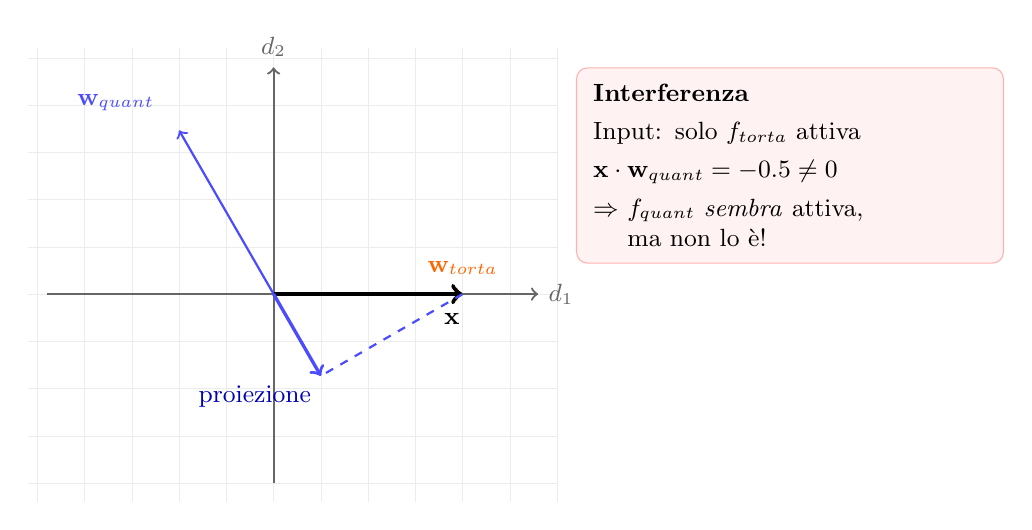
\begin{tikzpicture}[scale=2.4]
        % Griglia
        \draw[gray!15, very thin, step=0.25] (-1.3,-1.1) grid (1.5,1.3);
        
        % Assi (neuroni)
        \draw[->, thick, black!60] (-1.2,0) -- (1.4,0) node[right, font=\small] {$d_1$};
        \draw[->, thick, black!60] (0,-1.0) -- (0,1.2) node[above, font=\small] {$d_2$};
        
        % Direzioni delle feature
        \draw[->, thick, orange!80!red] (0,0) -- (1,0);
        \node[anchor=south, font=\small\bfseries, orange!80!red] at (1, 0.05) {$\mathbf{w}_{\text{torta}}$};
        
        \draw[->, thick, blue!70] (0,0) -- ({cos(120)},{sin(120)});
        \node[anchor=south east, font=\small\bfseries, blue!70] at ({cos(120)-0.08},{sin(120)+0.05}) {$\mathbf{w}_{\text{quant}}$};
        
        % Vettore x osservato (solo torta attiva)
        \draw[->, ultra thick, black] (0,0) -- (1,0);
        \node[anchor=north west, font=\small] at (0.85, -0.05) {$\mathbf{x}$};
        
        % Proiezione di x su w_quant
        \coordinate (proj) at ({cos(120)*(-0.5)},{sin(120)*(-0.5)});
        \draw[dashed, blue!70, thick] (1,0) -- (proj);
        \draw[->, blue!70, very thick] (0,0) -- (proj);
        \node[blue!70!black, font=\small, anchor=north east] at (proj) {proiezione};
        
        % Etichetta interferenza
        \node[anchor=north west, font=\small, align=left, text width=5cm, fill=red!5, draw=red!30, rounded corners, inner sep=6pt] at (1.6, 1.2) {
            \textbf{Interferenza}\\[0.3em]
            Input: solo $f_{\text{torta}}$ attiva\\[0.3em]
            $\mathbf{x} \cdot \mathbf{w}_{\text{quant}} = -0.5 \neq 0$\\[0.3em]
            $\Rightarrow$ $f_{\text{quant}}$ \textit{sembra} attiva,\\
            \phantom{$\Rightarrow$} ma non lo è!
        };
    \end{tikzpicture}
    \caption{Interferenza nella superposition. L'input contiene solo ``torta al cioccolato'' ($\mathbf{x} = \mathbf{w}_{\text{torta}}$), ma la proiezione su $\mathbf{w}_{\text{quant}}$ è non nulla ($-0.5$). La non-ortogonalità causa attivazioni spurie: feature inattive sembrano parzialmente attive.}
    \label{fig:interference}
\end{figure}

\paragraph{Il costo della compressione.}
L'interferenza è il prezzo da pagare per la superposition. Abbiamo guadagnato la possibilità di rappresentare più feature che neuroni, ma abbiamo perso la separabilità perfetta. Ogni volta che ``leggiamo'' l'attivazione di una feature, il segnale è contaminato dalle altre.
In formule, se proviamo a decodificare l'intensità $a_i$ tramite il prodotto scalare:
\begin{equation}
    \mathbf{x} \cdot \mathbf{w}_i = \sum_j a_j \, (\mathbf{w}_j \cdot \mathbf{w}_i) = a_i + \sum_{j \neq i} a_j \, (\mathbf{w}_j \cdot \mathbf{w}_i)
    \label{eq:interference}
\end{equation}
Il primo termine è il segnale che cerchiamo ($a_i$). Il secondo termine è il rumore di interferenza—la somma dei contributi di tutte le altre feature, pesati per quanto le loro direzioni sono ``allineate'' con $\mathbf{w}_i$. Solo se tutte le direzioni fossero ortogonali ($\mathbf{w}_j \cdot \mathbf{w}_i = 0$ per $j \neq i$), il rumore svanirebbe.
A questo punto la superposition sembra un pessimo affare: comprimiamo le feature, ma le rendiamo inseparabili. Perché mai una rete neurale dovrebbe adottare questa strategia?

\subsubsection{Perché funziona comunque: la sparsità delle feature}

L'interferenza sembra un problema grave: se ogni volta che decodifichiamo una feature otteniamo un segnale contaminato dalle altre, come può la rete funzionare correttamente? La risposta sta in un'osservazione empirica cruciale: \textbf{le feature sono sparse}.

\paragraph{Feature sparse nel mondo reale.}
Consideriamo i concetti che un modello linguistico deve rappresentare. ``Meccanica quantistica'' è rilevante solo in una minuscola frazione dei testi—articoli scientifici, manuali di fisica, discussioni specialistiche. ``Torta al cioccolato'' compare in contesti completamente diversi—ricette, blog culinari, menu di ristoranti. ``Legislazione fiscale'', ``errore di sintassi'', ``partita di calcio''—ciascun concetto ha il suo dominio ristretto.
In un dato input, solo \textit{pochi} concetti tra le migliaia possibili sono effettivamente pertinenti. Una frase sul calcio non menziona la meccanica quantistica; una ricetta di dolci non discute di legislazione fiscale. Le feature sono \textbf{sparse}: la maggior parte ha intensità $a_i = 0$ per la maggior parte degli input.
\paragraph{Sparsità e interferenza.}
Torniamo all'equazione dell'interferenza~\eqref{eq:interference}:
\begin{equation*}
    \mathbf{x} \cdot \mathbf{w}_i = a_i + \sum_{j \neq i} a_j \, (\mathbf{w}_j \cdot \mathbf{w}_i)
\end{equation*}
Il rumore di interferenza dipende dai prodotti $a_j \cdot (\mathbf{w}_j \cdot \mathbf{w}_i)$. Ma se la feature $f_j$ è inattiva ($a_j = 0$), il suo contributo al rumore è nullo—indipendentemente da quanto $\mathbf{w}_j$ sia allineata con $\mathbf{w}_i$.
Questo significa che \textit{l'interferenza si manifesta solo tra feature simultaneamente attive}. Se $f_{\text{torta}}$ e $f_{\text{quant}}$ non sono mai attive nello stesso input, possono condividere direzioni parzialmente sovrapposte senza mai interferire in pratica.
\begin{notebox}
\textbf{Sparsità e Superposition}\\
La superposition è vantaggiosa quando le feature sono sparse. Se ogni input attiva solo una piccola frazione delle feature totali, l'interferenza potenziale (dovuta alla non-ortogonalità) raramente si manifesta in pratica. La rete può ``stipare'' molte più feature di quanti siano i neuroni, accettando un piccolo rischio di interferenza nei rari casi di co-occorrenza.
\end{notebox}

\paragraph{Il trade-off sparsità-capacità.}
Emerge quindi un trade-off fondamentale, illustrato in Figura~\ref{fig:sparsity_superposition}. Al crescere della sparsità delle feature, la rete può permettersi di rappresentarne sempre di più nello stesso spazio:

\begin{enumerate}
    \item Sparsità 0\% (ogni feature sempre attiva): l'unica rappresentazione senza interferenza è quella disentangled—ogni feature su un asse dedicato. Se abbiamo $n$ neuroni, possiamo rappresentare al massimo $n$ feature.    
    \item Sparsità moderata (es. 50\%): le feature si attivano metà delle volte. Possiamo iniziare a usare direzioni non allineate agli assi, accettando interferenza occasionale. La capacità cresce oltre $n$.
    \item Sparsità alta (es. 90\%): le feature si attivano raramente. Possiamo ``stipare'' molte più feature come direzioni quasi-ortogonali—l'interferenza è rara perché le co-occorrenze sono rare. La capacità può crescere significativamente oltre $n$.
\end{enumerate}

\begin{figure}[htbp]
    \centering
    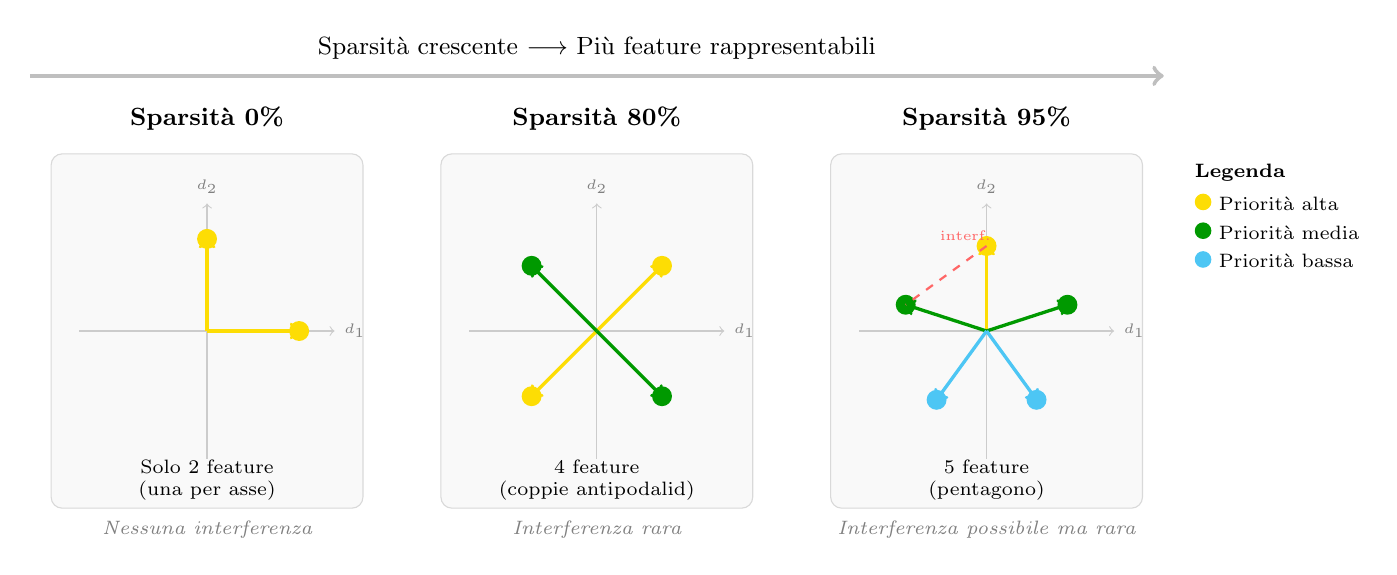
\begin{tikzpicture}[scale=0.9]    
        % === BOX 1: Sparsità 0% ===
        \draw[rounded corners, fill=gray!5, draw=gray!30] (-2.2,-2.5) rectangle (2.2,2.5);
        \node[font=\small\bfseries] at (0, 3) {Sparsità 0\%};     
        % Assi
        \draw[->, gray!40] (-1.8, 0) -- (1.8, 0) node[right, font=\tiny, gray] {$d_1$};
        \draw[->, gray!40] (0, -1.8) -- (0, 1.8) node[above, font=\tiny, gray] {$d_2$};
        % 2 feature sugli assi (ortogonali)
        \draw[->, very thick, yellow!80!orange] (0,0) -- (1.3,0);
        \draw[->, very thick, yellow!80!orange] (0,0) -- (0,1.3);
        \fill[yellow!80!orange] (1.3,0) circle (4pt);
        \fill[yellow!80!orange] (0,1.3) circle (4pt);
        \node[font=\scriptsize, align=center, text width=2.5cm] at (0, -2.1) {
            Solo 2 feature\\(una per asse)
        };
        \node[font=\scriptsize\itshape, gray] at (0, -2.8) {Nessuna interferenza};
        % === BOX 2: Sparsità 80% ===
        \begin{scope}[shift={(5.5,0)}]
            \draw[rounded corners, fill=gray!5, draw=gray!30] (-2.2,-2.5) rectangle (2.2,2.5);
            \node[font=\small\bfseries] at (0, 3) {Sparsità 80\%};
            % Assi
            \draw[->, gray!40] (-1.8, 0) -- (1.8, 0) node[right, font=\tiny, gray] {$d_1$};
            \draw[->, gray!40] (0, -1.8) -- (0, 1.8) node[above, font=\tiny, gray] {$d_2$};
            % 4 feature: due coppie antipodalid su assi obliqui
            % Coppia 1: asse a 45° (giallo)
            \draw[->, very thick, yellow!80!orange] (0,0) -- (0.92, 0.92);
            \draw[->, very thick, yellow!80!orange] (0,0) -- (-0.92, -0.92);
            \fill[yellow!80!orange] (0.92, 0.92) circle (4pt);
            \fill[yellow!80!orange] (-0.92, -0.92) circle (4pt);
            % Coppia 2: asse a -45° (verde)
            \draw[->, very thick, green!60!black] (0,0) -- (0.92, -0.92);
            \draw[->, very thick, green!60!black] (0,0) -- (-0.92, 0.92);
            \fill[green!60!black] (0.92, -0.92) circle (4pt);
            \fill[green!60!black] (-0.92, 0.92) circle (4pt);
            \node[font=\scriptsize, align=center, text width=2.8cm] at (0, -2.1) {
                4 feature\\(coppie antipodalid)
            };
            \node[font=\scriptsize\itshape, gray] at (0, -2.8) {Interferenza rara};
        \end{scope}
        % === BOX 3: Sparsità 95% ===
        \begin{scope}[shift={(11,0)}]
            \draw[rounded corners, fill=gray!5, draw=gray!30] (-2.2,-2.5) rectangle (2.2,2.5);
            \node[font=\small\bfseries] at (0, 3) {Sparsità 95\%};
            % Assi
            \draw[->, gray!40] (-1.8, 0) -- (1.8, 0) node[right, font=\tiny, gray] {$d_1$};
            \draw[->, gray!40] (0, -1.8) -- (0, 1.8) node[above, font=\tiny, gray] {$d_2$};
            % 5 feature come pentagono (72° tra loro)
            \draw[->, very thick, yellow!80!orange] (0,0) -- ({1.2*cos(90)}, {1.2*sin(90)});
            \fill[yellow!80!orange] ({1.2*cos(90)}, {1.2*sin(90)}) circle (4pt);
            \draw[->, very thick, green!60!black] (0,0) -- ({1.2*cos(162)}, {1.2*sin(162)});
            \fill[green!60!black] ({1.2*cos(162)}, {1.2*sin(162)}) circle (4pt);
            \draw[->, very thick, green!60!black] (0,0) -- ({1.2*cos(18)}, {1.2*sin(18)});
            \fill[green!60!black] ({1.2*cos(18)}, {1.2*sin(18)}) circle (4pt);
        
            \draw[->, very thick, cyan!70] (0,0) -- ({1.2*cos(234)}, {1.2*sin(234)});
            \fill[cyan!70] ({1.2*cos(234)}, {1.2*sin(234)}) circle (4pt);
            
            \draw[->, very thick, cyan!70] (0,0) -- ({1.2*cos(306)}, {1.2*sin(306)});
            \fill[cyan!70] ({1.2*cos(306)}, {1.2*sin(306)}) circle (4pt);
            
            % Linea di interferenza tra feature vicine
            \draw[dashed, red!60, thick] ({1.2*cos(90)}, {1.2*sin(90)}) -- ({1.2*cos(162)}, {1.2*sin(162)});
            \node[red!60, font=\tiny] at (-0.3, 1.35) {interf.};
            
            \node[font=\scriptsize, align=center, text width=2.8cm] at (0, -2.1) {
                5 feature\\(pentagono)
            };
            \node[font=\scriptsize\itshape, gray] at (0, -2.8) {Interferenza possibile ma rara};
        \end{scope}
        
        % Freccia sparsità crescente
        \draw[->, ultra thick, gray!50] (-2.5, 3.6) -- (13.5, 3.6);
        \node[font=\small, above] at (5.5, 3.7) {Sparsità crescente $\longrightarrow$ Più feature rappresentabili};
        
        % Legenda
        \node[anchor=north west, font=\scriptsize, align=left] at (13.8, 2.5) {
            \textbf{Legenda}\\[0.5em]
            \tikz\fill[yellow!80!orange] (0,0) circle (3pt); Priorità alta\\[0.3em]
            \tikz\fill[green!60!black] (0,0) circle (3pt); Priorità media\\[0.3em]
            \tikz\fill[cyan!70] (0,0) circle (3pt); Priorità bassa
        };
    \end{tikzpicture}
    \caption{Superposition al variare della sparsità (adattato da Elhage et al.~\parencite{elhage2022superposition}). Con sparsità 0\%, solo 2 feature ottengono assi dedicati (ortogonali). Con sparsità 80\%, 4 feature vengono rappresentate come coppie antipodalid su due assi obliqui (a 45° e -45°). Con sparsità 95\%, 5 feature sono distribuite come un pentagono—l'interferenza tra direzioni vicine è possibile, ma rara grazie alla bassa probabilità di co-occorrenza.}
    \label{fig:sparsity_superposition}
\end{figure}

\paragraph{La strategia ottimale della rete.}
Perché le reti neurali adottano la superposition? Perché è \textit{conveniente}. Il mondo del linguaggio naturale è dominato da feature sparse: la maggior parte dei concetti è rilevante solo in contesti specifici. In questa situazione, dedicare un neurone intero a ogni concetto sarebbe uno spreco—quel neurone resterebbe inattivo per la stragrande maggioranza degli input.
La superposition permette di sfruttare la capacità della rete in modo più efficiente: ``ricicla'' gli stessi neuroni per feature diverse, confidando nel fatto che raramente serviranno contemporaneamente. È una forma di \textbf{compressione lossy}—perdiamo la perfetta separabilità, ma guadagniamo enormemente in capacità rappresentativa.
Questo spiega come BERT possa rappresentare decine di migliaia di concetti con soli 768 neuroni: le feature sono codificate come direzioni quasi-ortogonali, e la sparsità naturale del linguaggio garantisce che l'interferenza, pur possibile in linea di principio, sia rara in pratica.


\subsubsection{Conseguenze della superposition}

Ricapitoliamo. Le reti neurali come BERT rappresentano molte più feature di quanti siano i neuroni disponibili, codificandole come direzioni quasi-ortogonali nello spazio delle attivazioni. Questa strategia—la superposition—è resa possibile dalla sparsità naturale delle feature: poiché la maggior parte dei concetti è raramente attiva, l'interferenza tra direzioni non ortogonali si manifesta di rado.

La superposition è una soluzione elegante al paradosso della capacità, ma ha un costo: l'\textbf{opacità}.

\paragraph{Il problema dell'opacità.}
L'informazione semantica è presente nell'embedding $\mathbf{x}$—codificata nelle direzioni $\mathbf{w}_i$ e nelle intensità $a_i$. Ma questa informazione è \textit{inaccessibile}:

\begin{itemize}
    \item \textbf{Non conosciamo le direzioni} $\mathbf{w}_i$: la rete le ha apprese durante l'addestramento, ma non ce le rivela esplicitamente. Sono ``sepolte'' nei pesi del modello.
    
    \item \textbf{Non conosciamo le intensità} $a_i$: anche se conoscessimo le direzioni, l'interferenza impedirebbe un recupero esatto.
    
    \item \textbf{Non conosciamo nemmeno quante feature ci siano}: il numero $m$ di concetti rappresentati dalla rete è ignoto.
\end{itemize}

Il risultato è che l'embedding $\mathbf{x}$ appare come un vettore opaco di 768 numeri, privo di significato interpretabile. Sappiamo che contiene informazione semantica ricca—il modello funziona—ma non possiamo estrarla né ispezionarla.

\paragraph{Implicazioni pratiche.}
Questa opacità ha conseguenze concrete per chi sviluppa e utilizza modelli linguistici:

\begin{itemize}
    \item \textbf{Debugging}: quando il modello commette un errore, non possiamo identificare \textit{quale} feature ha causato il problema. L'errore potrebbe derivare da un concetto mal rappresentato, da interferenza tra feature, o da un'attivazione spuria—ma non abbiamo modo di distinguere questi casi.
    
    \item \textbf{Controllo}: non possiamo modificare selettivamente il comportamento del modello. Se volessimo, ad esempio, rimuovere un bias o amplificare l'attenzione verso certi concetti, non sapremmo su quali ``leve'' agire.
    
    \item \textbf{Fiducia}: in applicazioni critiche—medicina, diritto, finanza—è difficile fidarsi di un sistema che non possiamo ispezionare. La superposition rende i modelli potenti ma imperscrutabili.
    
    \item \textbf{Allineamento}: più in generale, se non comprendiamo \textit{come} un modello rappresenta l'informazione, non possiamo garantire che si comporti in modo sicuro e prevedibile. Questo è il cuore del cosiddetto \textit{problema dell'allineamento}~\parencite{elhage2022superposition}.
\end{itemize}

\paragraph{Una via d'uscita?}
La situazione sembra senza speranza: la superposition è ciò che rende i modelli potenti, ma anche ciò che li rende opachi. Possiamo avere l'una senza l'altra?

L'osservazione chiave è che la \textit{sparsità} gioca un ruolo duplice. Da un lato, è ciò che \textit{permette} la superposition: le feature possono sovrapporsi perché raramente sono attive insieme. Dall'altro, la sparsità è anche una proprietà \textit{desiderabile} per l'interpretabilità: se solo poche feature sono attive per ogni input, diventa più facile identificarle e comprenderle.

Questo suggerisce una strategia: invece di cercare di decodificare direttamente le direzioni $\mathbf{w}_i$ nascoste in BERT, potremmo \textit{costruire un nuovo spazio} dove le feature corrispondano esplicitamente agli assi—uno spazio dove ogni coordinata $h_i$ rappresenti l'intensità di una feature $f_i$ specifica. Se questo spazio fosse sufficientemente grande (più dimensioni che feature) e le attivazioni fossero sparse (poche $h_i$ non nulle per input), avremmo ottenuto il meglio di entrambi i mondi: la ricchezza rappresentativa della superposition con l'interpretabilità del disentanglement.

Questo è esattamente ciò che gli \textbf{Sparse Autoencoders} si propongono di fare. Nella prossima sezione esploreremo come la sparsità, lo stesso principio che rende possibile la superposition, possa essere sfruttata per \textit{invertirla}.


\subsection{L'approccio sparse: intuizione e motivazione}
\label{subsec:sparse_approach}

La sezione precedente ha mostrato come la superposition permetta alle reti neurali di rappresentare migliaia di feature in poche centinaia di dimensioni, al prezzo dell'opacità. L'informazione semantica è presente—codificata come direzioni $\mathbf{w}_i$ nello spazio degli embedding—ma è inaccessibile: non conosciamo le direzioni, non conosciamo le intensità $a_i$, e anche se le conoscessimo, l'interferenza ne impedirebbe un recupero esatto.

Ma la stessa proprietà che rende possibile la superposition—la sparsità delle feature—suggerisce una via d'uscita.

\subsubsection{Invertire la superposition}

Ricordiamo la situazione. In BERT, un embedding $\mathbf{x} \in \mathbb{R}^{768}$ codifica l'informazione relativa a molte feature $f_1, f_2, \dots, f_m$ simultaneamente:
\begin{equation}
    \mathbf{x} = \sum_{i=1}^{m} a_i \, \mathbf{w}_i
\end{equation}
dove $m \gg 768$. Le direzioni $\mathbf{w}_i$ sono sconosciute, le intensità $a_i$ sono sconosciute, e le direzioni non sono ortogonali. Questo è il problema.

L'obiettivo è costruire una rappresentazione dove l'informazione sia \textit{esplicita}:
\begin{itemize}
    \item Ogni feature $f_i$ corrisponde a un \textbf{asse} dedicato—non a una direzione obliqua
    \item L'intensità $a_i$ è \textbf{leggibile} direttamente come coordinata lungo quell'asse
    \item Le feature sono \textbf{separate}—nessuna interferenza
\end{itemize}

In altre parole, vogliamo passare da uno spazio dove le feature sono \textit{direzioni sconosciute} a uno spazio dove le feature sono \textit{assi noti}. Vogliamo una rappresentazione $\mathbf{h}$ tale che:
\begin{equation}
    h_i \neq 0 \quad \Longleftrightarrow \quad \text{la feature } f_i \text{ è attiva nell'input}
\end{equation}

Questo è esattamente il mondo ideale disentangled che abbiamo descritto all'inizio del capitolo—ma con una differenza cruciale: non possiamo ottenerlo in 768 dimensioni, perché le feature sono molte di più.

\paragraph{L'intuizione chiave.}
La superposition esiste perché BERT deve rappresentare $m$ feature in $n < m$ dimensioni. Le feature vengono ``compresse'' come direzioni oblique perché non c'è abbastanza spazio per dare a ciascuna un asse dedicato.

Ma cosa succederebbe se avessimo \textit{abbastanza spazio}? Se costruissimo un nuovo spazio con $q \geq m$ dimensioni—una per ogni feature—il problema della compressione svanirebbe. Ogni feature potrebbe avere il suo asse, e non ci sarebbe bisogno di superposition.

Questo è il punto di partenza: per invertire la superposition, dobbiamo \textbf{espandere} lo spazio, non comprimerlo.

\subsubsection{Lo spazio overcomplete}

L'idea è semplice: se 768 dimensioni non bastano per dare a ogni feature un asse dedicato, costruiamo uno spazio più grande. Invece di cercare di decodificare le direzioni nascoste in $\mathbb{R}^{768}$, proiettiamo l'embedding $\mathbf{x}$ in un nuovo spazio $\mathbb{R}^q$ con $q \gg 768$.

Concretamente, definiamo un \textbf{encoder}—una funzione $\text{enc}_\theta$—che mappa l'embedding originale in questo spazio espanso:
\begin{equation}
    \mathbf{h} = \text{enc}_\theta(\mathbf{x}), \qquad \mathbf{h} \in \mathbb{R}^q, \quad q \gg 768
\end{equation}

Questo spazio si dice \textbf{overcomplete}: ha più dimensioni dello spazio di partenza. Se BERT usa 768 dimensioni e le feature da rappresentare sono, diciamo, 50.000, allora scegliamo $q = 50.000$ o più. In questo spazio c'è abbastanza ``posto'' perché ogni feature abbia potenzialmente un asse dedicato.
\begin{figure}[htbp]
    \centering
    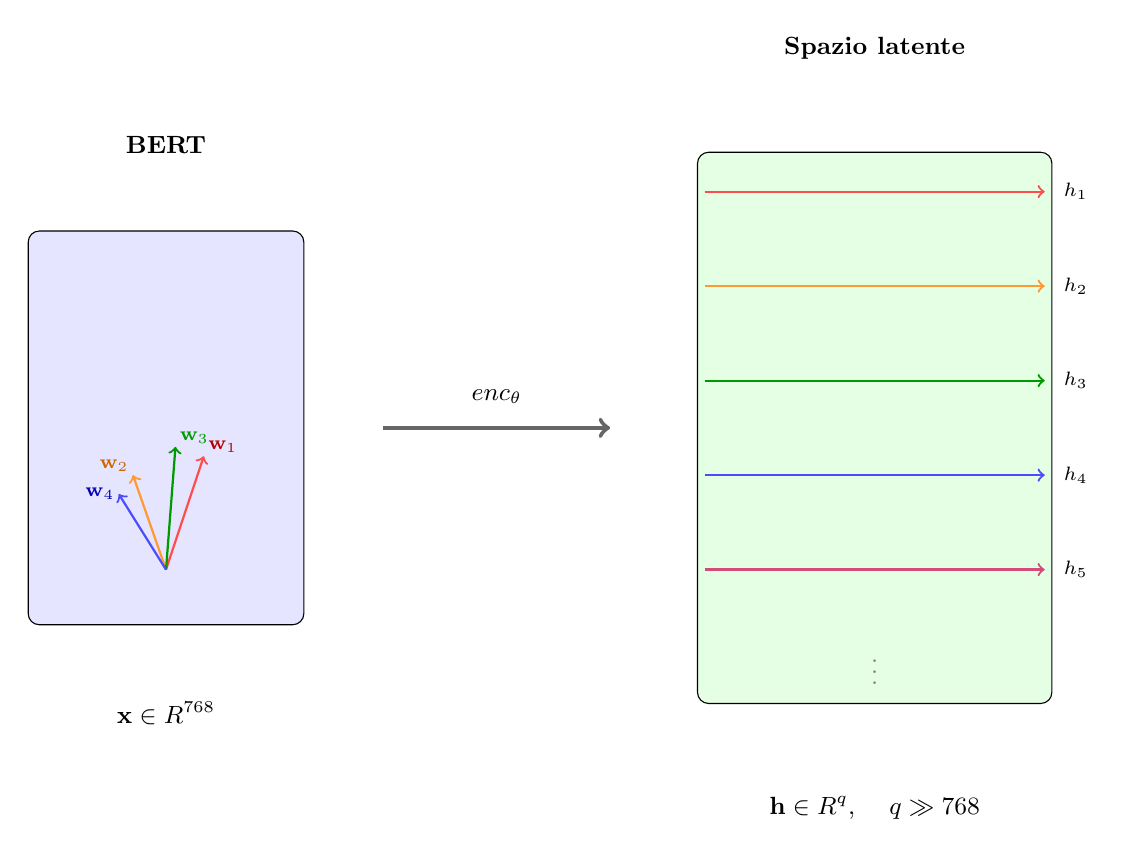
\begin{tikzpicture}[scale=1.2]
        % Spazio originale (box più grande)
        \node[draw, rectangle, minimum width=3.5cm, minimum height=5cm, fill=blue!10, rounded corners] (x) at (0,0) {};
        \node[above, font=\small\bfseries] at (0, 2.8) {BERT};
        
        % Frecce interne (direzioni oblique, mescolate) - ACCORCIATE
        \coordinate (origin) at (0, -1.5);
        % Ho ridotto le lunghezze (i valori nel ++) di circa il 30-40%
        \draw[->, thick, red!70] (origin) -- ++(0.4, 1.2);
        \draw[->, thick, orange!80] (origin) -- ++(-0.35, 1.0);
        \draw[->, thick, green!60!black] (origin) -- ++(0.1, 1.3);
        \draw[->, thick, blue!70] (origin) -- ++(-0.5, 0.8);
        
        % Etichette riposizionate per seguire le frecce più corte
        \node[font=\scriptsize, red!70!black] at (0.6, -0.2) {$\mathbf{w}_1$};
        \node[font=\scriptsize, orange!80!black] at (-0.55, -0.4) {$\mathbf{w}_2$};
        \node[font=\scriptsize, green!60!black] at (0.3, -0.1) {$\mathbf{w}_3$};
        \node[font=\scriptsize, blue!70!black] at (-0.7, -0.7) {$\mathbf{w}_4$};
        
        \node[below, font=\small] at (0, -2.8) {$\mathbf{x} \in \mathbb{R}^{768}$};
        
        % Encoder
        \draw[->, ultra thick, black!60] (2.3, 0) -- (4.7, 0);
        \node[above, font=\small] at (3.5, 0.15) {$\text{enc}_\theta$};
        
        % Spazio overcomplete (box più grande)
        \node[draw, rectangle, minimum width=4.5cm, minimum height=7cm, fill=green!10, rounded corners] (h) at (7.5,0) {};
        \node[above, font=\small\bfseries] at (7.5, 3.8) {Spazio latente};
        
        % Assi orizzontali (feature separate)
        \foreach \y/\c/\lab in {2.5/red!70/$h_1$, 1.5/orange!80/$h_2$, 0.5/green!60!black/$h_3$, -0.5/blue!70/$h_4$, -1.5/purple!70/$h_5$} {
            \draw[->, thick, \c] (5.7, \y) -- (9.3, \y);
            \node[font=\scriptsize, right] at (9.4, \y) {\lab};
        }
        
        \node[font=\small, gray] at (7.5, -2.5) {$\vdots$};
        
        \node[below, font=\small] at (7.5, -3.8) {$\mathbf{h} \in \mathbb{R}^{q}$, \quad $q \gg 768$};
        
    \end{tikzpicture}
    \caption{Dall'embedding compresso allo spazio overcomplete. A sinistra, BERT codifica le feature come direzioni oblique $\mathbf{w}_i$ in 768 dimensioni—mescolate e sconosciute (superposition). A destra, l'encoder $\text{enc}_\theta$ proietta in uno spazio con $q \gg 768$ dimensioni, dove ogni feature può avere un asse dedicato: la coordinata $h_i$ indica direttamente l'intensità della feature $f_i$.}
    \label{fig:overcomplete_space}
\end{figure}

\paragraph{Espandere non basta.}
L'espansione dimensionale è necessaria, ma non sufficiente. Nulla garantisce, a priori, che l'encoder $\text{enc}_\theta$ organizzi lo spazio $\mathbf{h}$ nel modo desiderato. Potremmo ritrovarci con 50.000 dimensioni in cui l'informazione è ancora mescolata e opaca—solo distribuita su più numeri.
Per ottenere una rappresentazione dove $h_i$ corrisponda effettivamente alla feature $f_i$, serve un \textbf{vincolo} che guidi l'apprendimento. Questo vincolo è la sparsità.

\subsubsection{La sparsità come chiave}

Abbiamo costruito uno spazio più grande—ma questo, da solo, non basta. Senza vincoli, l'encoder potrebbe distribuire l'informazione in modo arbitrario su tutte le $q$ dimensioni, producendo una rappresentazione altrettanto opaca di quella di partenza, solo più grande.

Il vincolo che trasforma lo spazio overcomplete in una rappresentazione interpretabile è la \textbf{sparsità}: per ogni input, solo \textit{poche} coordinate di $\mathbf{h}$ possono essere attive.

L'intuizione è semplice. Se l'encoder può ``accendere'' solo un piccolo numero di dimensioni per rappresentare un input, ma deve comunque catturare tutta l'informazione necessaria alla ricostruzione, allora ogni dimensione è costretta a \textbf{specializzarsi}. Non può permettersi di codificare miscele ambigue di concetti—deve diventare un ``rilevatore'' dedicato a una specifica feature semantica.

È lo stesso principio che rende possibile la superposition, ma usato al contrario: là, la sparsità delle feature permetteva di comprimerle in poche dimensioni; qui, imponiamo sparsità alle attivazioni per forzare la separazione delle feature in dimensioni distinte.

Quando l'addestramento converge, il risultato è una rappresentazione dove:
\begin{itemize}
    \item Ogni coordinata $h_i$ corrisponde a una feature $f_i$ specifica
    \item $h_i \neq 0$ indica che la feature è attiva nell'input
    \item Il valore di $h_i$ indica l'intensità della feature
\end{itemize}

Abbiamo invertito la superposition: le direzioni sconosciute $\mathbf{w}_i$ sono diventate assi noti $h_i$.

I dettagli tecnici di come imporre la sparsità e addestrare questo tipo di modelli saranno presentati nel Capitolo~\ref{sec:prisma}, dove introdurremo PRISMA. Per ora, ci basta l'intuizione fondamentale: \textit{spazio grande + attivazioni sparse = feature separate}.
%https://claude.ai/chat/a893ee36-8c08-401b-b4be-f02cb99770a5

\subsection{Feature interpretability: cosa significa "capire" una feature}
\label{subsec:feature_interpretability}

Abbiamo visto come gli Sparse Autoencoders possano trasformare le rappresentazioni opache di BERT in uno spazio dove ogni coordinata $h_i$ corrisponde, idealmente, a una feature semantica $f_i$. Ma cosa significa, concretamente, che una feature è \textit{interpretabile}? E come possiamo verificare che le dimensioni apprese abbiano davvero un significato comprensibile?

\subsubsection{Quando una feature è interpretabile?}

Nel contesto della superposition, le feature erano codificate come direzioni $\mathbf{w}_i$ nello spazio di BERT. Queste direzioni esistevano—la rete le usava—ma erano inaccessibili: non potevamo né identificarle né attribuire loro un significato.

Con gli SAE, la situazione cambia. Ogni dimensione $h_i$ dello spazio latente dovrebbe corrispondere a una feature distinta. Ma ``corrispondere a una feature'' non basta: vogliamo che questa feature sia \textbf{interpretabile}—che un essere umano possa guardarla e capire cosa rappresenta.

\begin{notebox}
\textbf{Feature interpretabile}\\
Una feature si dice \textit{interpretabile} quando è possibile assegnarle un'\textbf{etichetta semantica} coerente—una descrizione in linguaggio naturale che cattura il concetto codificato. Ad esempio:
\begin{itemize}
    \item ``Questa feature si attiva per riferimenti a cibi dolci''
    \item ``Questa feature rileva menzioni di città europee''
    \item ``Questa feature risponde a espressioni di incertezza''
\end{itemize}
L'etichetta deve essere \textit{predittiva}: conoscendola, dovremmo poter anticipare in quali contesti la feature si attiverà.
\end{notebox}

L'interpretabilità è quindi una proprietà che riguarda la relazione tra la feature e la comprensione umana. Una feature potrebbe essere ``reale'' nel senso che cattura una regolarità statistica dei dati, ma non interpretabile se questa regolarità non corrisponde a nessun concetto che sappiamo nominare.

\paragraph{Interpretabile vs monosematico.}
È importante distinguere due proprietà correlate ma distinte:
\begin{itemize}
    \item Una feature è \textbf{monosematica} se si attiva per un \textit{unico} tipo di concetto (anziché mescolare concetti diversi come nella polisemantia).
    \item Una feature è \textbf{interpretabile} se quel concetto unico è \textit{comprensibile} per un umano.
\end{itemize}

Una feature potrebbe essere monosematica—attivarsi sempre e solo per lo stesso tipo di pattern—ma non interpretabile, se quel pattern non corrisponde a nulla che sappiamo descrivere. Viceversa, l'interpretabilità implica tipicamente la monosemantia: se possiamo dare un'etichetta coerente, la feature probabilmente cattura un concetto unitario.

L'obiettivo degli SAE è produrre feature che siano \textit{entrambe} le cose: monosemantiche (grazie alla sparsità) e interpretabili (verificabile empiricamente).

\subsubsection{Il processo di interpretazione}

Come si determina, in pratica, se una feature è interpretabile? Il processo segue una logica semplice: osservare \textit{quando} la feature si attiva e cercare \textit{cosa hanno in comune} quegli input.

\paragraph{Passo 1: trovare le attivazioni massime.}
Data una dimensione $h_i$ dello spazio latente, il primo passo è identificare gli input del dataset che la attivano maggiormente. Si cercano i testi per cui $h_i$ assume i valori più alti—i casi in cui la feature ``risponde'' con più forza.

Ad esempio, analizzando la dimensione $h_{42}$ su un corpus di testi, potremmo trovare che i dieci input con attivazione massima sono:
\begin{enumerate}
    \item ``La torta al cioccolato era deliziosa''
    \item ``Aggiungi zucchero all'impasto''
    \item ``La ricetta prevede burro e farina''
    \item ``Il dolce è stato un successo''
    \item ``Mescola gli ingredienti per la crema''
    \item[] $\vdots$
\end{enumerate}

\paragraph{Passo 2: identificare i pattern comuni.}
Il secondo passo è cercare regolarità tra questi input. Cosa li accomuna? Nel nostro esempio, il pattern è evidente: tutti riguardano la preparazione di dolci o ingredienti da pasticceria.

A volte il pattern è chiaro; altre volte è più sfumato o sorprendente. Una feature potrebbe attivarsi per ``frasi che contengono numeri seguiti da unità di misura'', o per ``espressioni di cortesia formale'', o per ``riferimenti a eventi passati''. Il compito dell'interprete è trovare la descrizione che meglio cattura la regolarità.

\paragraph{Passo 3: assegnare un'etichetta.}
Una volta identificato il pattern, si formula un'etichetta descrittiva:
\begin{center}
    \textit{``La feature $h_{42}$ si attiva per riferimenti a dolci e pasticceria''}
\end{center}

L'etichetta deve essere sufficientemente precisa da essere \textit{predittiva}: leggendo un nuovo testo, dovremmo poter anticipare se la feature si attiverà o meno. Un'etichetta troppo vaga (``testi su cose buone'') o troppo specifica (``solo torte al cioccolato con burro'') non è utile.

\paragraph{Visualizzare le feature.}
Il processo diventa più intuitivo quando si visualizzano le attivazioni. Una pratica comune è mostrare gli input ordinati per attivazione decrescente, evidenziando le parole o frasi che sembrano ``triggerare'' la feature. Questo permette di cogliere pattern che una semplice lista non renderebbe evidenti.
\begin{figure}[htbp]
    \centering
    \begin{tikzpicture}[scale=1]
        % Box principale (fisso a 12x6cm, centro 0,0)
        \node[draw, rectangle, minimum width=12cm, minimum height=6cm, fill=gray!5, rounded corners] at (0,0) {};
        
        % Titolo
        \node[font=\small\bfseries] at (0, 2.5) {Feature $h_{42}$: attivazioni massime};
        
        % --- Blocco Sinistro: Esempi ---
        % Spostati leggermente a destra (da -5.5 a -5.2) per migliorare il margine sinistro
        \node[anchor=west, font=\small] at (-5.2, 1.5) {1. \; ``La \colorbox{yellow!50}{torta al cioccolato} era deliziosa''};
        \node[anchor=west, font=\small] at (-5.2, 0.8) {2. \; ``Aggiungi \colorbox{yellow!50}{zucchero} all'impasto''};
        \node[anchor=west, font=\small] at (-5.2, 0.1) {3. \; ``La \colorbox{yellow!50}{ricetta} prevede \colorbox{yellow!50}{burro} e \colorbox{yellow!50}{farina}''};
        \node[anchor=west, font=\small] at (-5.2, -0.6) {4. \; ``Il \colorbox{yellow!50}{dolce} è stato un successo''};
        \node[anchor=west, font=\small] at (-5.2, -1.3) {5. \; ``Mescola gli \colorbox{yellow!50}{ingredienti} per la \colorbox{yellow!50}{crema}''};
        
        % --- Blocco Destro: Barre di attivazione ---
        % Spostate leggermente a sinistra (l'inizio x passa da 3 a 2.6) per compattare
        \foreach \y/\w in {1.5/2.2, 0.8/2.0, 0.1/1.8, -0.6/1.6, -1.3/1.4} {
            \fill[orange!70] (2.6, \y-0.15) rectangle (2.6+\w, \y+0.15);
        }
        % Etichetta piccola sopra le barre (spostata di conseguenza)
        \node[font=\tiny, gray] at (3.7, 1.9) {attivazione $h_{42}$};
        
        % --- NUOVA POSIZIONE ETICHETTA ---
        % Posizionata in basso, centrata rispetto al blocco delle barre sopra di essa
        \node[font=\small\itshape, align=center, draw=gray!30, fill=white, rounded corners, inner sep=5pt] (labelNode) at (3.7, -2.3) {Etichetta interpretata:\\``Dolci e pasticceria''};
        
        % Freccia curva che scende dalle barre all'etichetta
        \draw[->, thick, gray, -{Stealth[length=3mm]}] (3.7, -1.5) to[out=-90, in=90] (labelNode.north);
        
    \end{tikzpicture}
    \caption{Interpretazione della feature $h_{42}$. Gli esempi con le attivazioni più alte (barre arancioni) condividono un tema comune. Osservando questo pattern, si assegna un'etichetta semantica descrittiva, posizionata in basso.}
    \label{fig:feature_interpretation_centered}
\end{figure}

\paragraph{Automatizzare con i Large Language Models.}
Il processo che abbiamo descritto—trovare attivazioni massime, identificare pattern, assegnare etichette—è concettualmente semplice. Ma c'è un problema pratico: la \textbf{scala}.

Uno Sparse Autoencoder tipico produce migliaia o decine di migliaia di feature. Interpretarle manualmente, una per una, richiederebbe settimane o mesi di lavoro—un approccio che semplicemente non scala. E anche volendo, l'interpretazione umana è soggettiva: due analisti potrebbero proporre etichette diverse per la stessa feature.

La soluzione è delegare il compito a un sistema che possieda le capacità necessarie: leggere testi, identificare pattern semantici, formulare descrizioni in linguaggio naturale. Queste sono esattamente le capacità dei \textbf{Large Language Models}.

L'idea è usare un LLM come ``interprete automatico''. Dato un insieme di input che attivano fortemente una dimensione $h_i$, chiediamo al modello:
\begin{center}
    \textit{``Cosa hanno in comune questi testi? Descrivi in una frase il concetto che li accomuna.''}
\end{center}

Il modello analizza gli esempi e produce un'etichetta—esattamente come farebbe un analista umano, ma in una frazione del tempo e in modo sistematico. Migliaia di feature possono essere interpretate in pochi minuti, rendendo finalmente possibile esplorare l'intero spazio latente di uno Sparse Autoencoder.

Questo approccio sarà al centro del Capitolo~\ref{sec:prisma}, dove presenteremo PRISMA e mostreremo come l'interpretazione automatica via LLM consenta di trasformare le rappresentazioni opache di BERT in un catalogo di concetti semantici leggibili e navigabili.
